\noindent\textbf{C.1. Free--free beam.}
\begin{figure}[H]
\centering
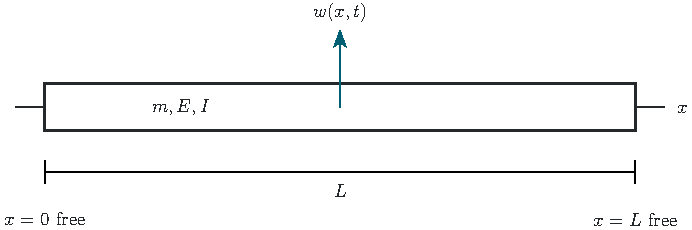
\includegraphics[width=0.75\linewidth]{figures/generated/solutions/C1-free-beam.pdf}
\caption{Uniform beam free at both ends, with transverse displacement $w(x,t)$.}
\end{figure}
The uniform beam has length $L$, bending stiffness $EI$, mass per unit length $m$, and free ends at $x=0$ and $x=L$. The end moment and shear vanish, giving
\[
M(0,t)=M(L,t)=0,\qquad V(0,t)=V(L,t)=0,
\]
or $W''(0)=W'''(0)=W''(L)=W'''(L)=0$ for constant $EI$. With $a=(EI/m)^{1/4}$, the course beam equation is $w_{tt}+a^4 w_{xxxx}=0$. Set $w=W(x)e^{-i\omega t}$ and $\gamma^4=\omega^2/a^4$. The spatial solution is
\[
W=C_1\cosh(\gamma x)+C_2\sinh(\gamma x)+C_3\cos(\gamma x)+C_4\sin(\gamma x).
\]
The left-end conditions give $C_3=C_1$ and $C_4=C_2$. With $z=\gamma L$, the remaining boundary conditions become
\[
\begin{bmatrix}
\cosh z-\cos z&\sinh z-\sin z\\
\sinh z+\sin z&\cosh z-\cos z
\end{bmatrix}
\begin{bmatrix}C_1\\C_2\end{bmatrix}=0.
\]
The determinant is $2(1-\cosh z\cos z)$. The solution $C_1=C_2=0$ is the trivial zero-displacement solution. A nonzero flexible mode requires $\cosh z\cos z=1$, with positive roots $4.73004,7.85320,10.9956,14.1372,17.2788,\ldots$. The two zero-frequency rigid-body modes are constant translation and rotation. The flexible eigenvalues give
\[
\gamma_j=z_j/L,\qquad\omega_j=a^2(z_j/L)^2,\qquad f_j=\omega_j/(2\pi),
\]
and an unnormalized flexible mode is
\[
W_j(x)=\cosh(\gamma_jx)+\cos(\gamma_jx)
-\beta_j[\sinh(\gamma_jx)+\sin(\gamma_jx)],\quad
\beta_j=\frac{\cosh z_j-\cos z_j}{\sinh z_j-\sin z_j}.
\]
Normalize each mode by $\phi_j=W_j/\sqrt{\int_0^L W_j^2dx}$ for the unweighted convention. Distinct modes satisfy $\int_0^L\phi_i\phi_j\,dx=\delta_{ij}$.

For $C_2=1$, the left-end equations give $C_4=1$, $C_1=C_3=-1/\beta_j$ with the $\beta_j$ defined above. Thus the same mode may be written as
\[
W_j=\sinh(\gamma_jx)+\sin(\gamma_jx)
-\frac{1}{\beta_j}\left[\cosh(\gamma_jx)+\cos(\gamma_jx)\right].
\]
The scalar amplitude is arbitrary. For numerical root finding, $\cos z-\operatorname{sech}z=0$ is equivalent to the characteristic equation and avoids overflow. At large $j$, $z_j\approx(j+\tfrac12)\pi$. The first ten positive flexible roots are compared below.
\begin{center}
\begin{tabular}{rrr}\toprule
$j$ & $z_j$ from \texttt{fzero} & $(j+1/2)\pi$\\\midrule
1&4.730040745&4.712388980\\
2&7.853204624&7.853981634\\
3&10.995607838&10.995574288\\
4&14.137165491&14.137166941\\
5&17.278759657&17.278759595\\
6&20.420352246&20.420352248\\
7&23.561944902&23.561944902\\
8&26.703537556&26.703537556\\
9&29.845130209&29.845130209\\
10&32.986722863&32.986722863\\
\bottomrule\end{tabular}
\end{center}
For $j\ge 6$, the discrepancy is at most $2.71\times10^{-9}$ in this table. The MATLAB script calculates the ten roots using bounded intervals.
\lstinputlisting[style=hwmatlab,caption={Free--free beam eigenvalues.}]{matlab/C1.m}
